\newpage
\section{Model}\label{model}
\subsection{Delegates}
Figure \ref{Delegate} shows the number of delegates awarded after each primary/caucus per candidate. The results are displayed for each state until Super Tuesday.  
\begin{figure}[H]
    \centering
    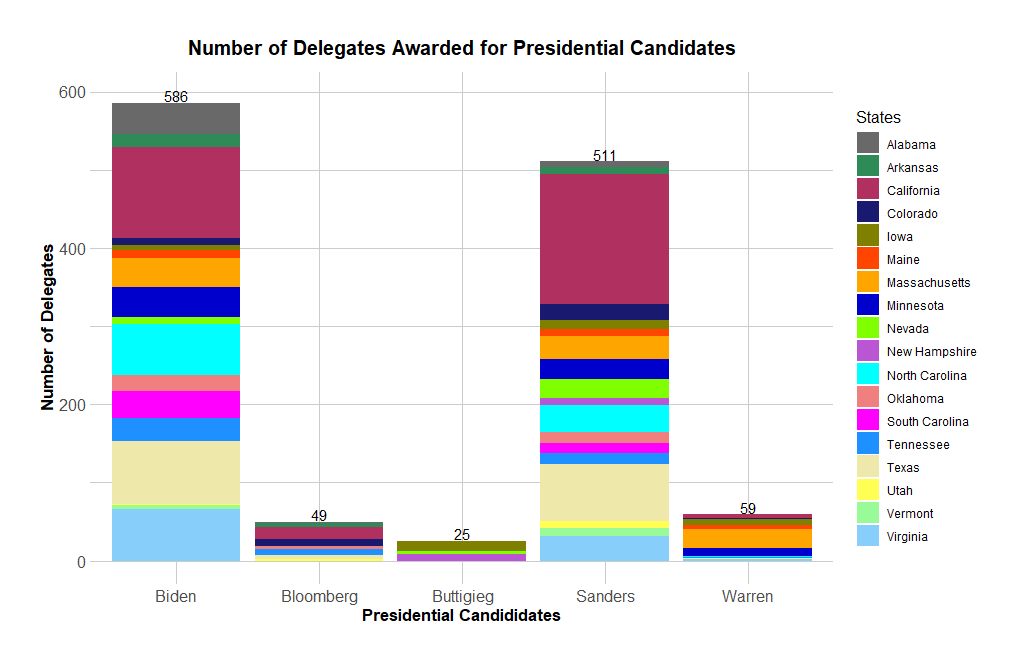
\includegraphics[width=0.7\textwidth]{figures/Delegate.png}
    \caption{Delegate}
    \label{Delegate}
\end{figure}

\subsection{Polling}
The poll data is collected and plotted for top five democratic candidates(Biden, Sanders, Warren, Bloomberg and Buttigieg). Data is plotted for both A rated and for all the polls as displayed in figures \ref{Updated-Polling-Data-1}, \ref{A-rated-polls} and \ref{All-rated-polls}. 
\begin{figure}[H]
    \centering
    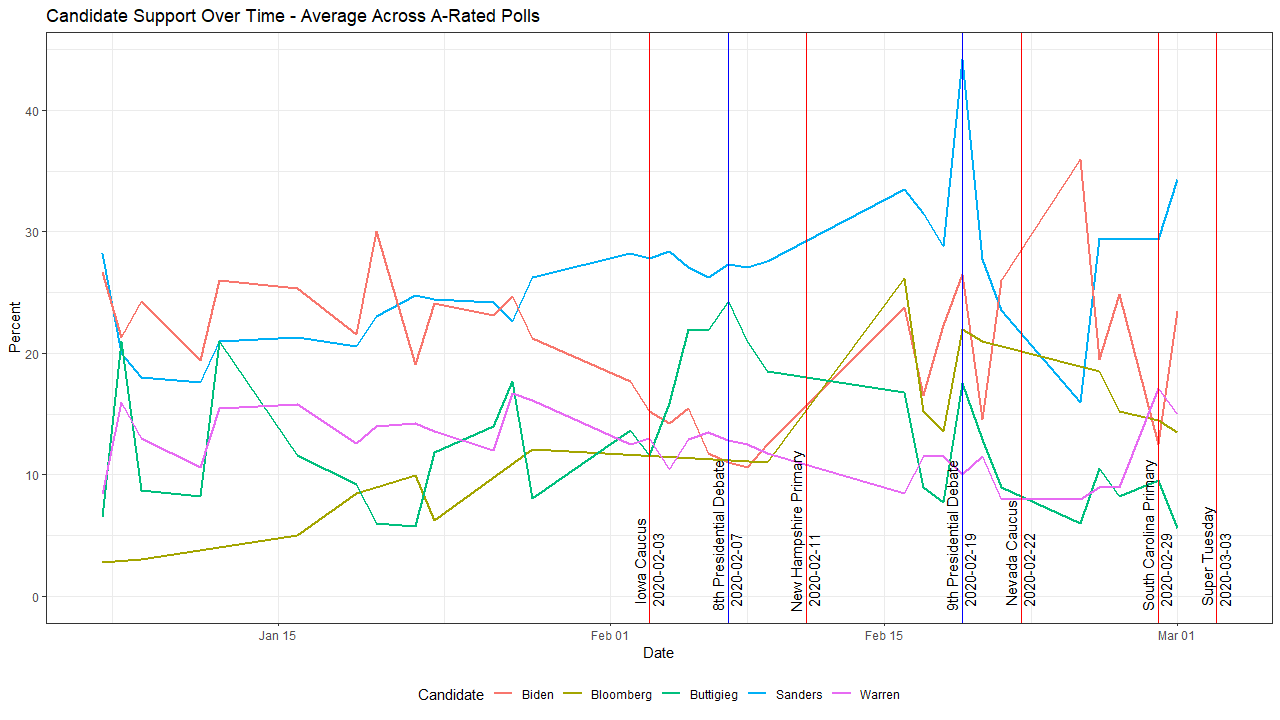
\includegraphics[width=0.7\textwidth]{figures/long-A-rated-polls.png}
    \caption{Updated Polling Data}
    \label{Updated-Polling-Data-1}
\end{figure}
Figure \ref{A-rated-polls} displays the support for candidates collected from A rated polls. At the end of  South Carolina Primary , it is observed that Sanders has the highest percentage of support is the highest and Buttigieg has the lowest percentage of support.  
\begin{figure}[H]
    \centering
    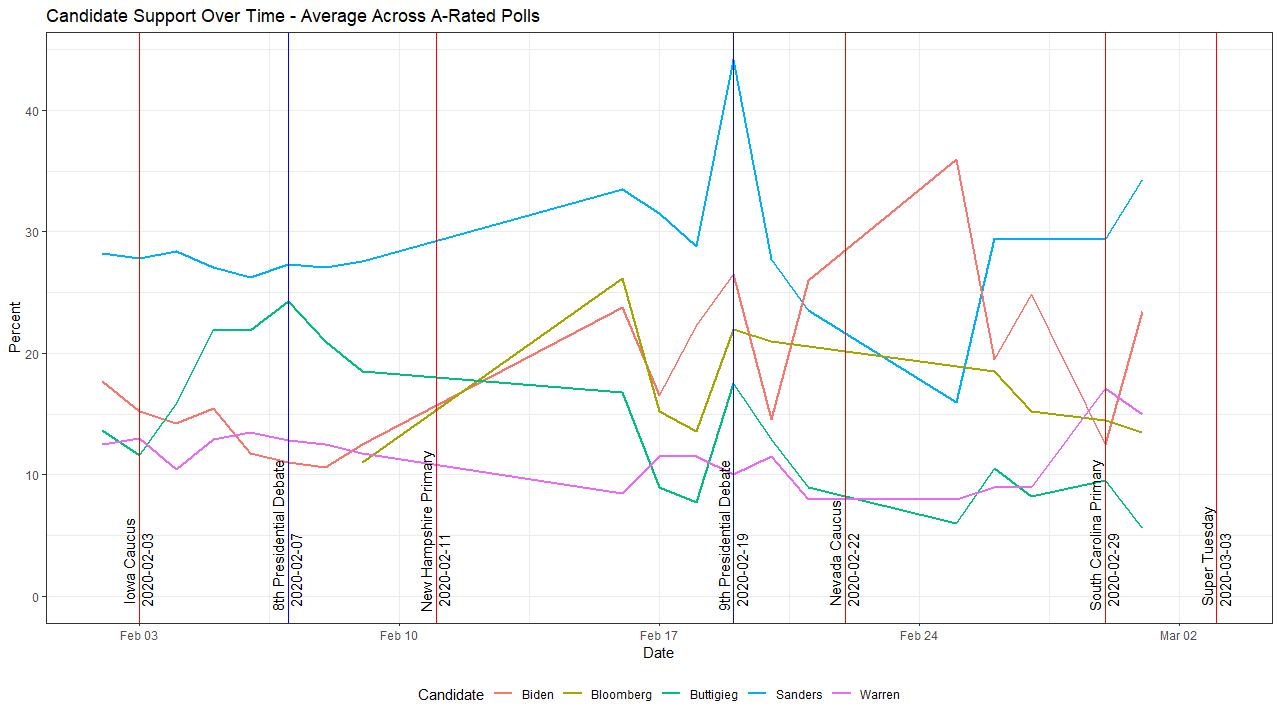
\includegraphics[width=0.9\textwidth]{figures/A-rated-polls.png}
    \caption{A Rated Polls}
    \label{A-rated-polls}
\end{figure}

\begin{figure}[H]
    \centering
    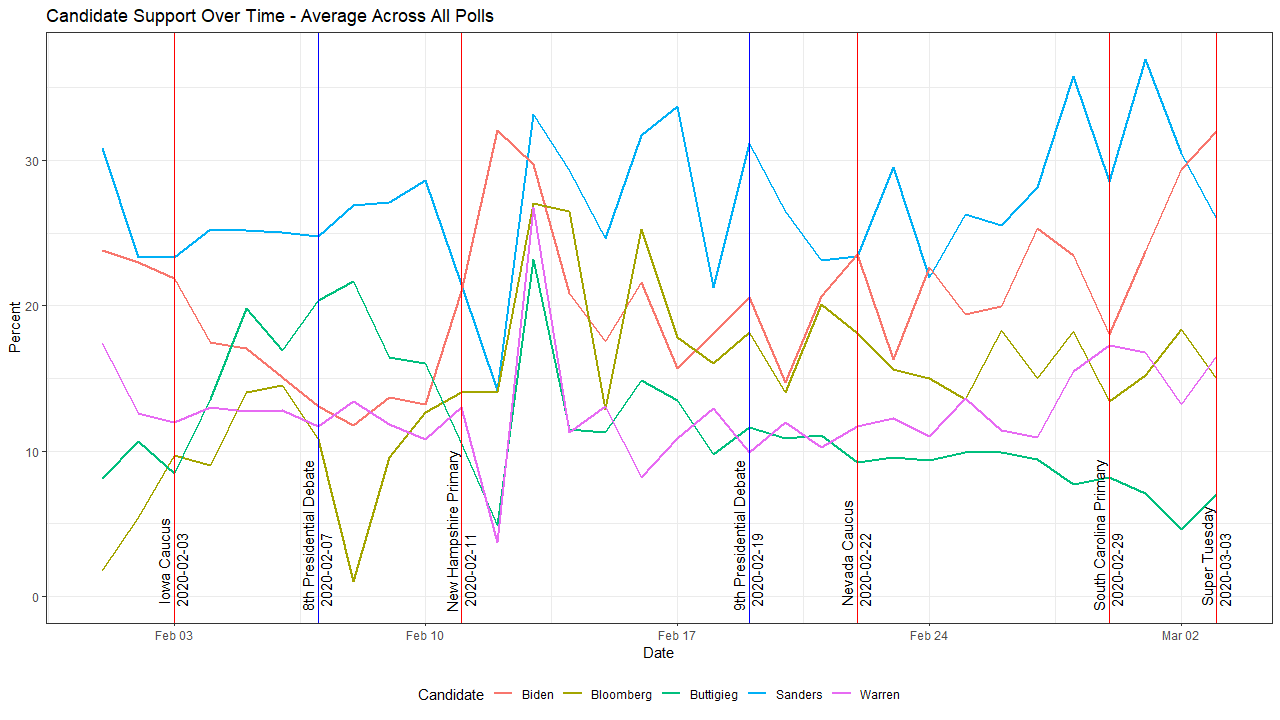
\includegraphics[width=0.9\textwidth]{figures/All-rated-polls.png}
    \caption{All-rated-polls}
    \label{All-rated-polls}
\end{figure}

Figures \ref{scatter-A-rated} and \ref{scatter-all} display scatter plot with curve smoothing for top three candidates(Biden, Warren and Sanders)
\begin{figure}[H]
    \centering
    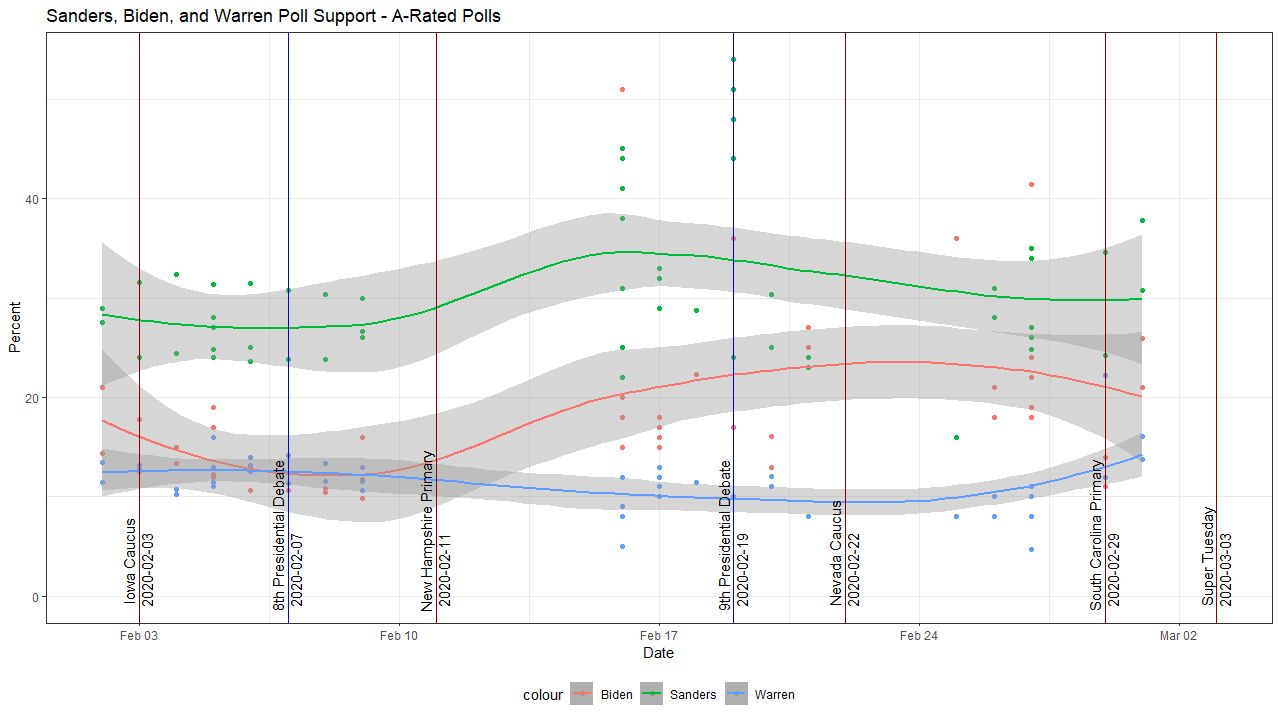
\includegraphics[width=0.9\textwidth]{figures/scatter-A-rated.png}
    \caption{scatter-A-rated}
    \label{scatter-A-rated}
\end{figure}

\begin{figure}[H]
    \centering
    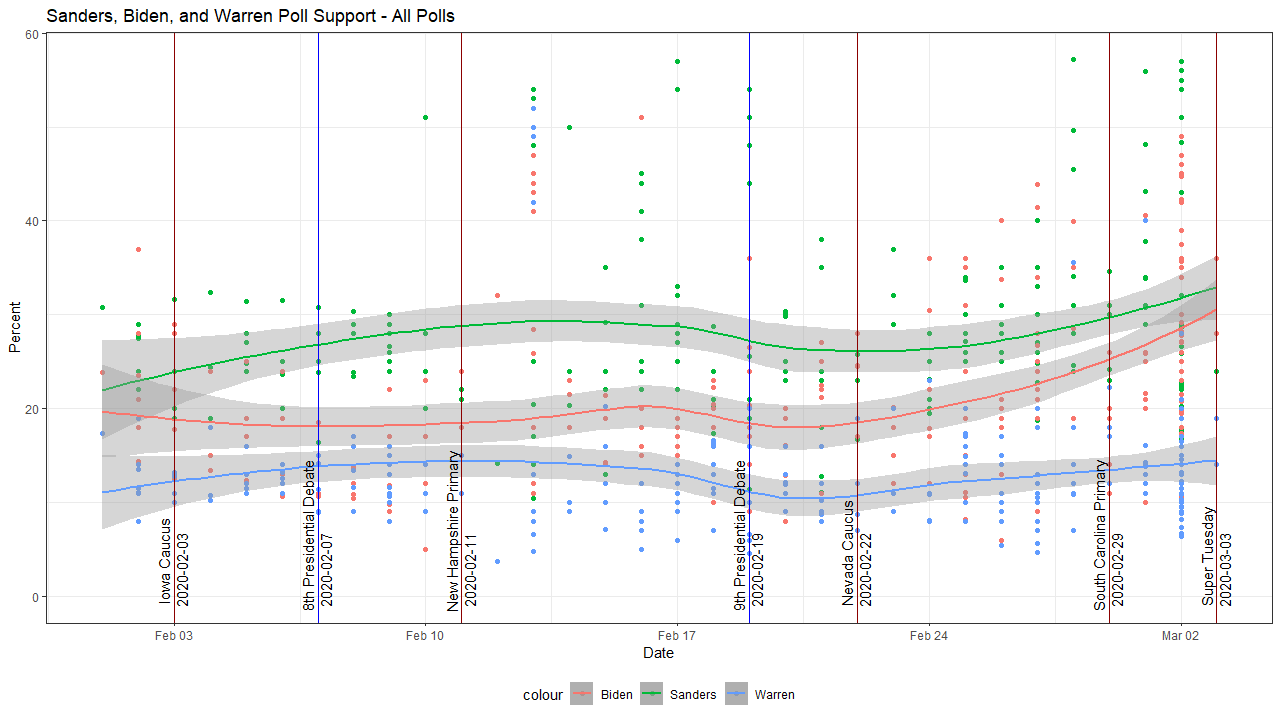
\includegraphics[width=0.9\textwidth]{figures/scatter-all.png}
    \caption{scatter-all}
    \label{scatter-all}
\end{figure}

\begin{figure}[H]
    \centering
    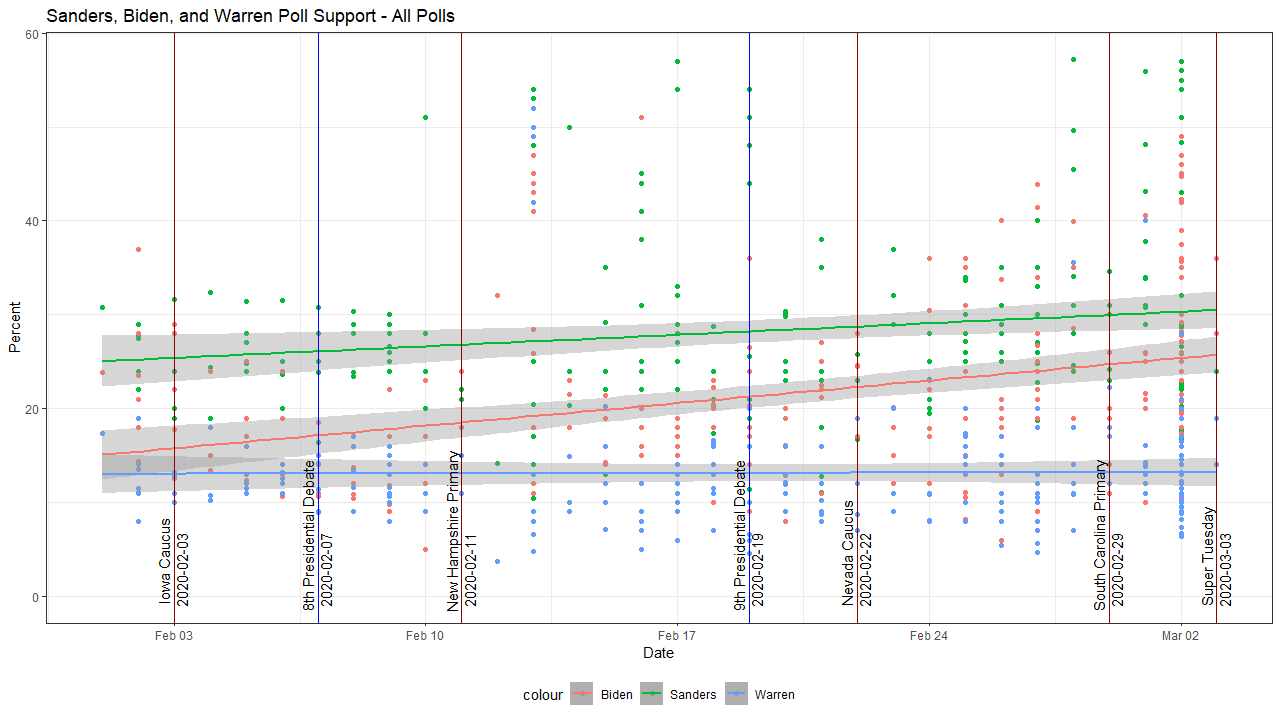
\includegraphics[width=0.9\textwidth]{figures/scatter-all-linear.png}
    \caption{scatter-all-linear}
    \label{scatter-all-linear}
\end{figure}

\subsection{Spending}
Figures \ref{MoneyspendinAds} to \ref{Nevada} shows the amount of money spent on advertisements state wise(Iowa, New Hampshire and Nevada). 

\begin{figure}[H]
    \centering
    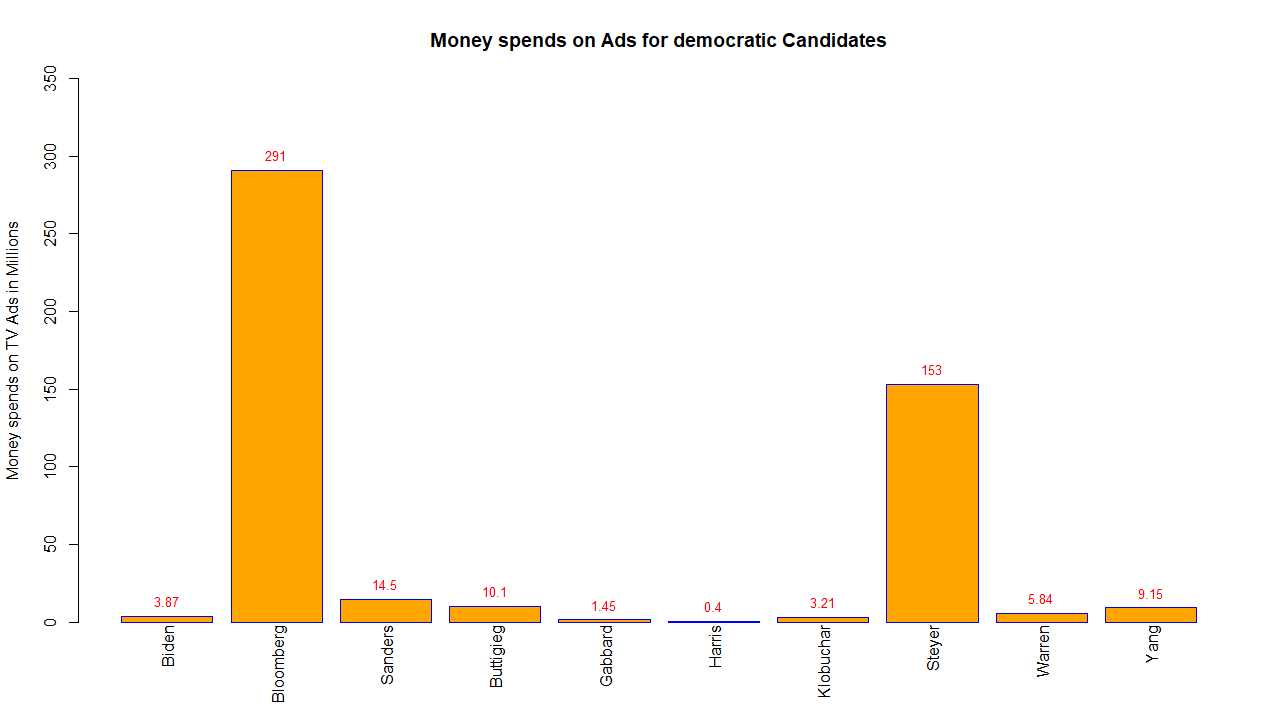
\includegraphics[width=0.9\textwidth]{figures/MoneyspendinAds.png}
    \caption{Money spending on Ads}
    \label{MoneyspendinAds}
\end{figure}

\begin{figure}[H]
    \centering
    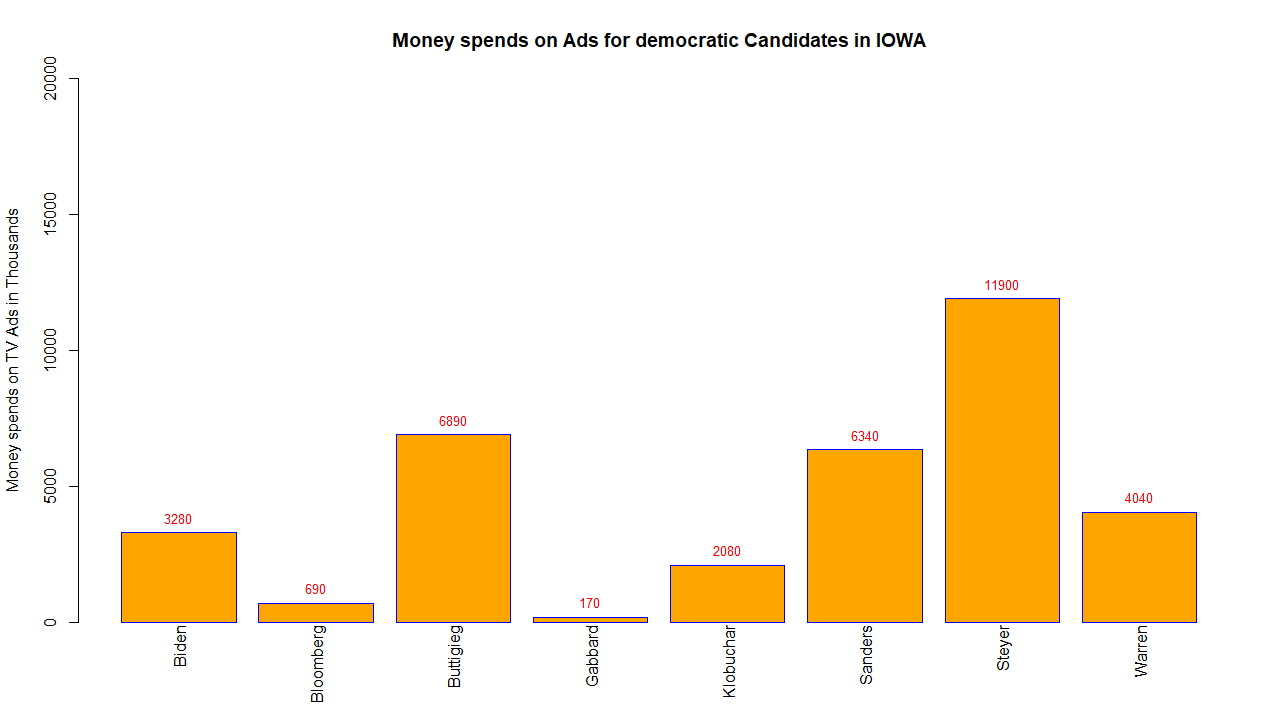
\includegraphics[width=0.9\textwidth]{figures/IOWA.png}
    \caption{Money spending on Ads in Iowa}
    \label{IOWA}
\end{figure}

\begin{figure}[H]
    \centering
    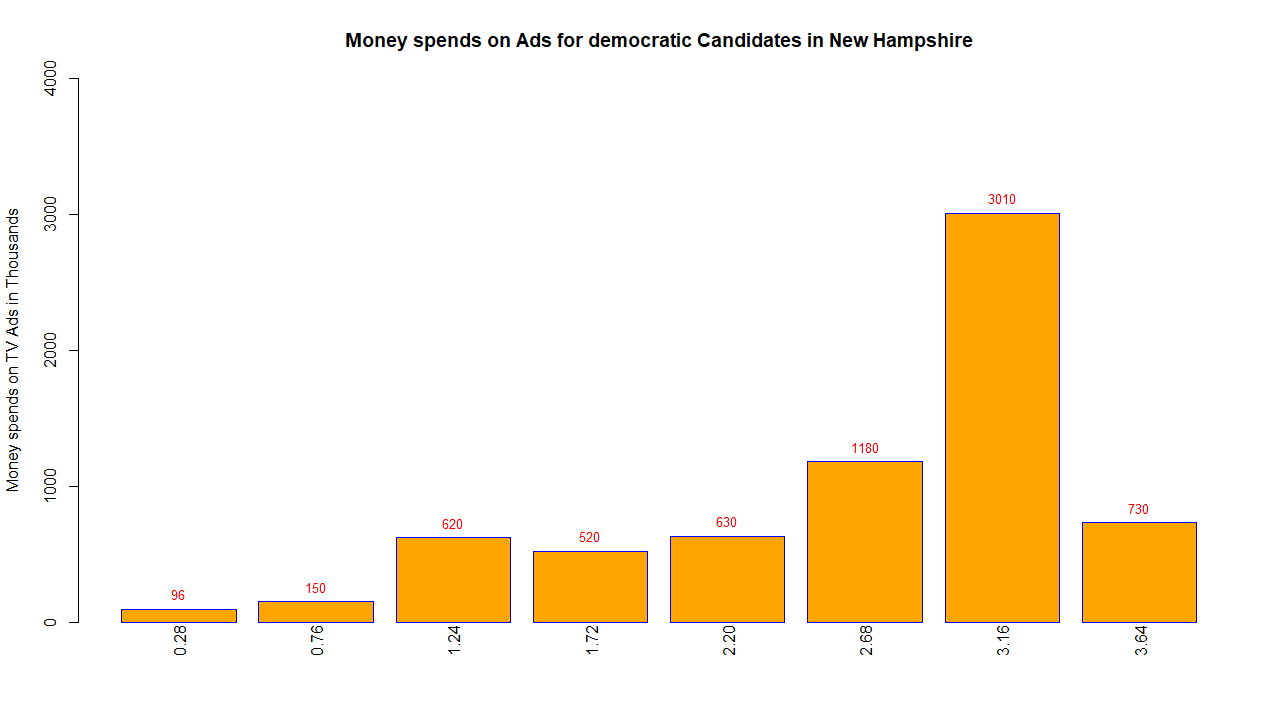
\includegraphics[width=0.9\textwidth]{figures/Newhampshire.png}
    \caption{Money spending on Ads in New Hampshire}
    \label{Newhampshire}
\end{figure}

\begin{figure}[H]
    \centering
    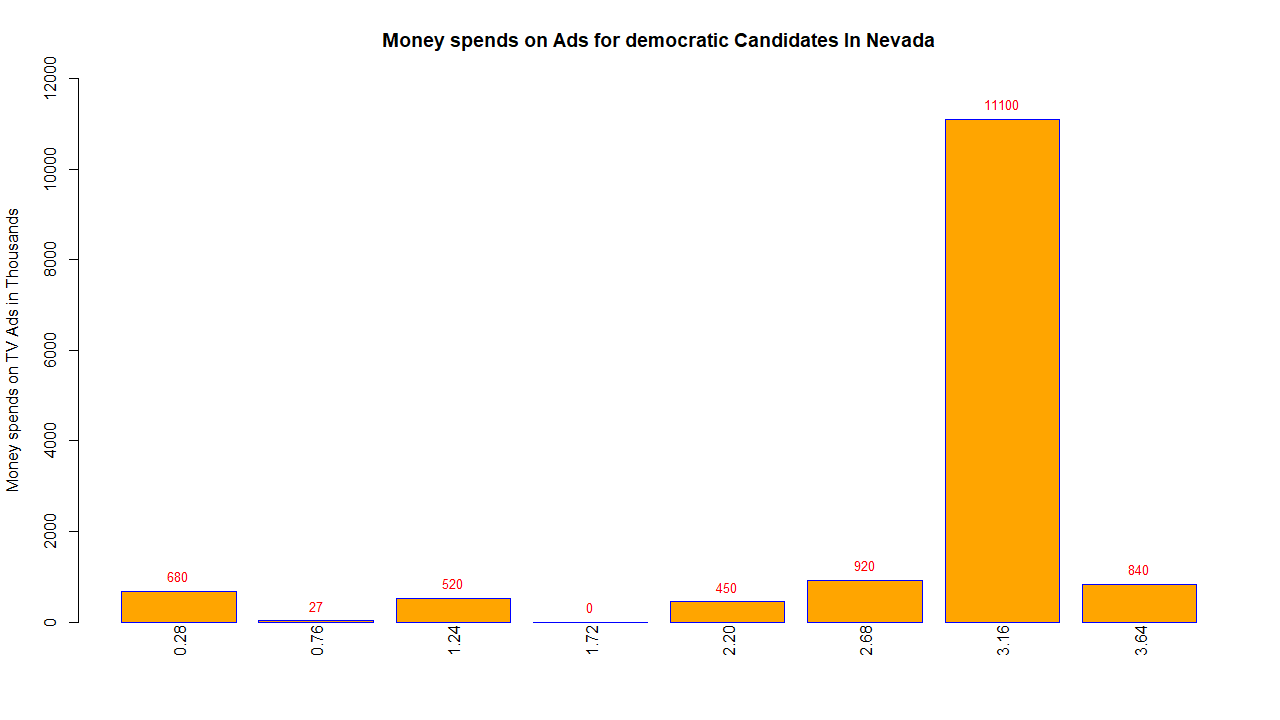
\includegraphics[width=0.9\textwidth]{figures/Nevada.png}
    \caption{Money spending on Ads in Nevada}
    \label{Nevada}
\end{figure}

\subsection{Funding}
Figures \ref{Total} to \ref{Others} shows funding from small and big donors,  self funding and funding from other sources.  
\begin{figure}[H]
    \centering
    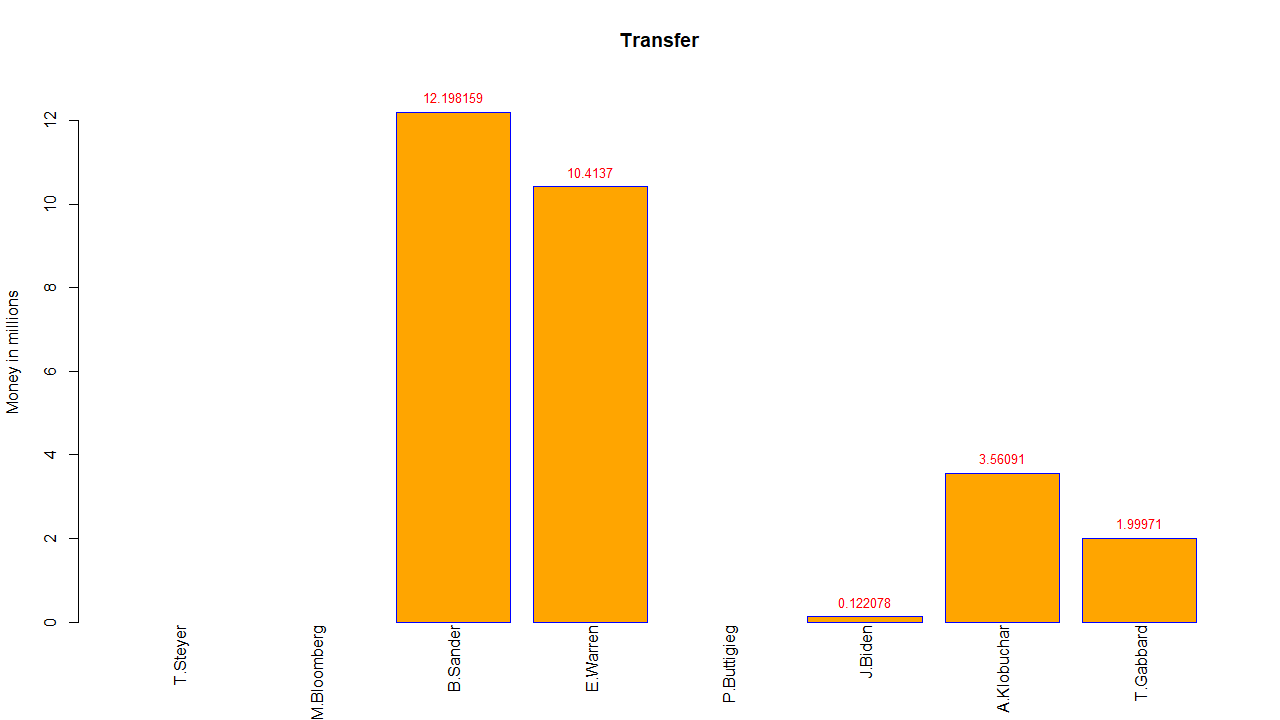
\includegraphics[width=0.9\textwidth]{figures/Total.png}
    \caption{Total Funding}
    \label{Total}
\end{figure}

\begin{figure}[H]
    \centering
    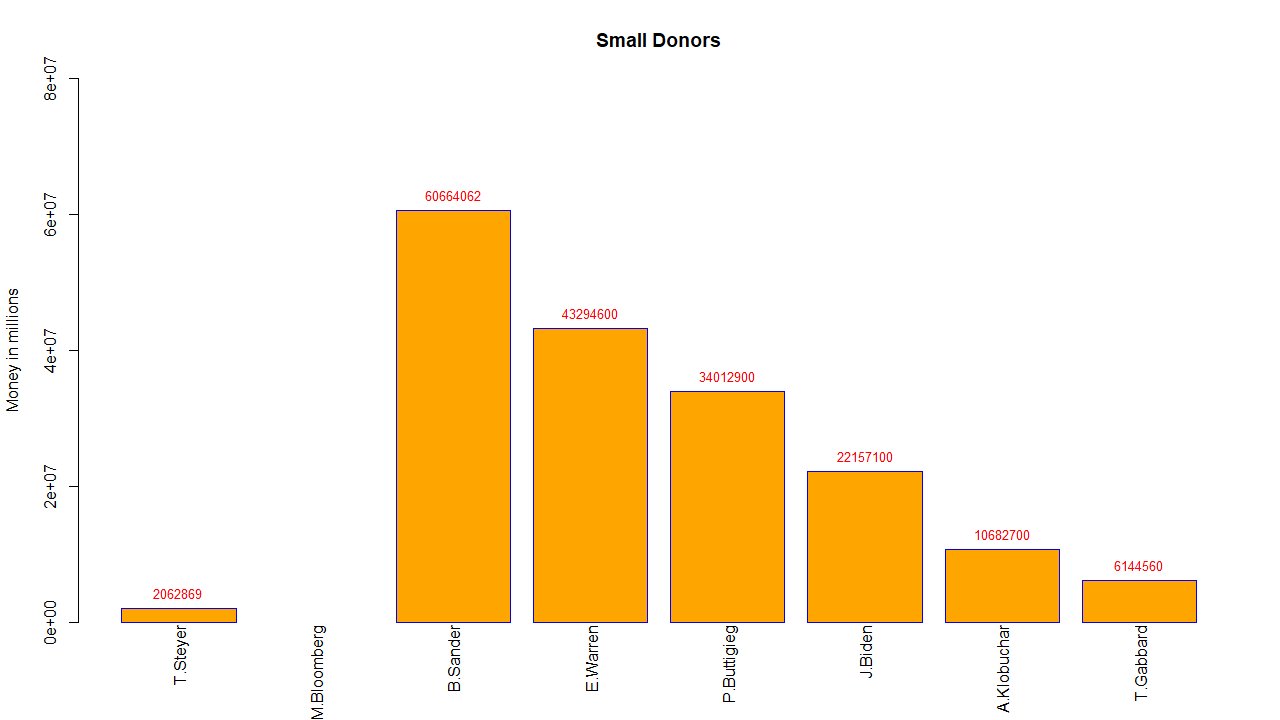
\includegraphics[width=0.9\textwidth]{figures/Small Donors.png}
    \caption{Small Donors Funding}
    \label{Small Donors}
\end{figure}

\begin{figure}[H]
    \centering
    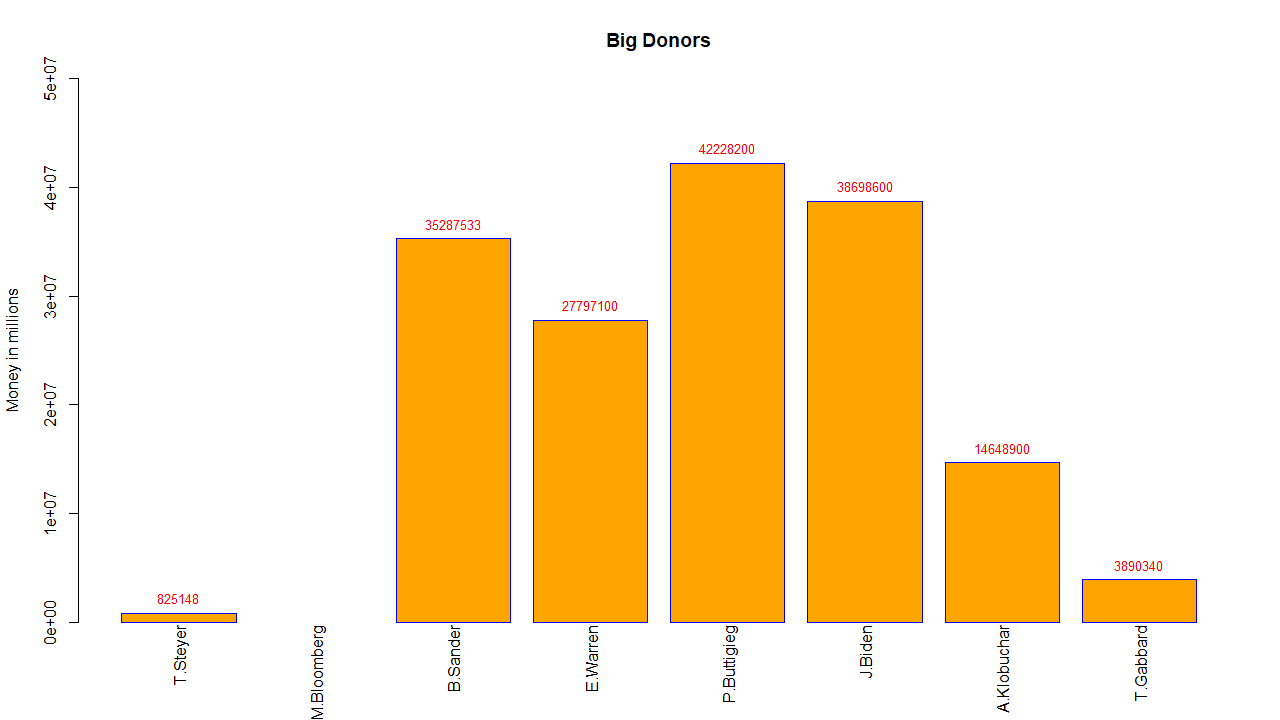
\includegraphics[width=0.9\textwidth]{figures/Bigdonor.png}
    \caption{Big donors Funding}
    \label{Bigdonor}
\end{figure}

\begin{figure}[H]
    \centering
    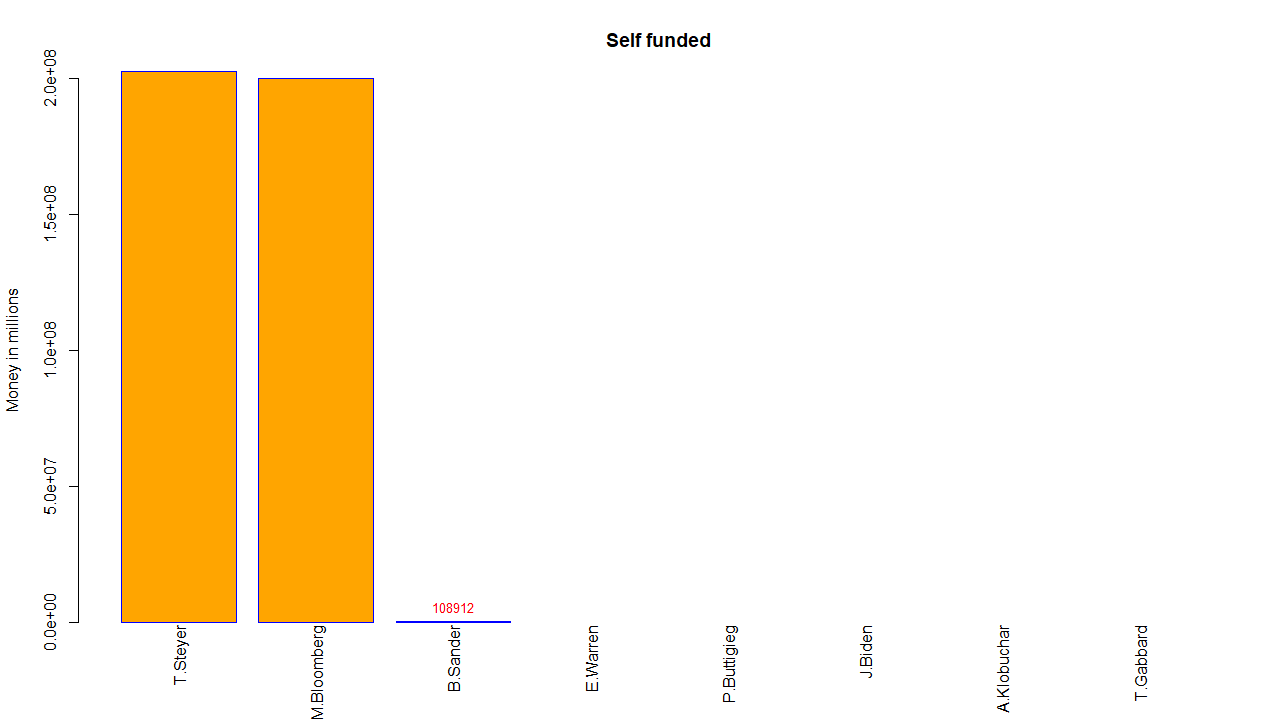
\includegraphics[width=0.9\textwidth]{figures/Selffunnded.png}
    \caption{Self funnded Funding}
    \label{Selffunnded}
\end{figure}

\begin{figure}[H]
    \centering
    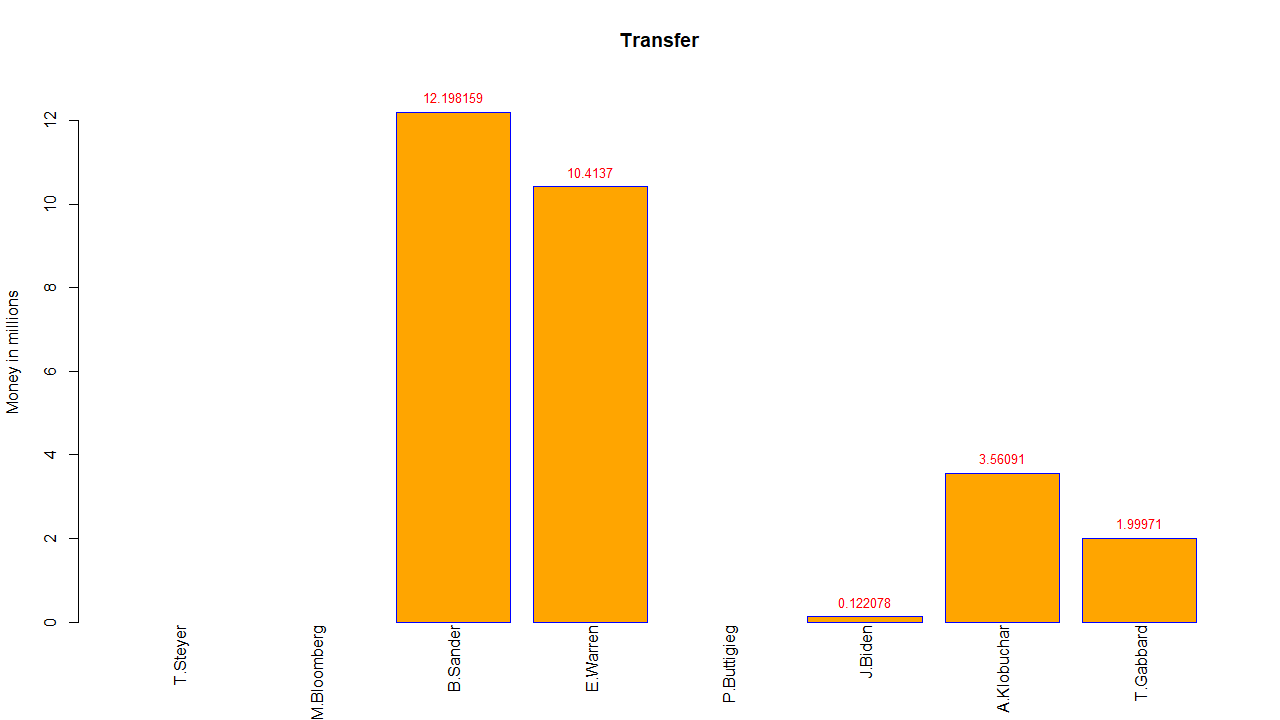
\includegraphics[width=0.9\textwidth]{figures/Transfer.png}
    \caption{Transfer Funding}
    \label{Transfer}
\end{figure}

\begin{figure}[H]
    \centering
    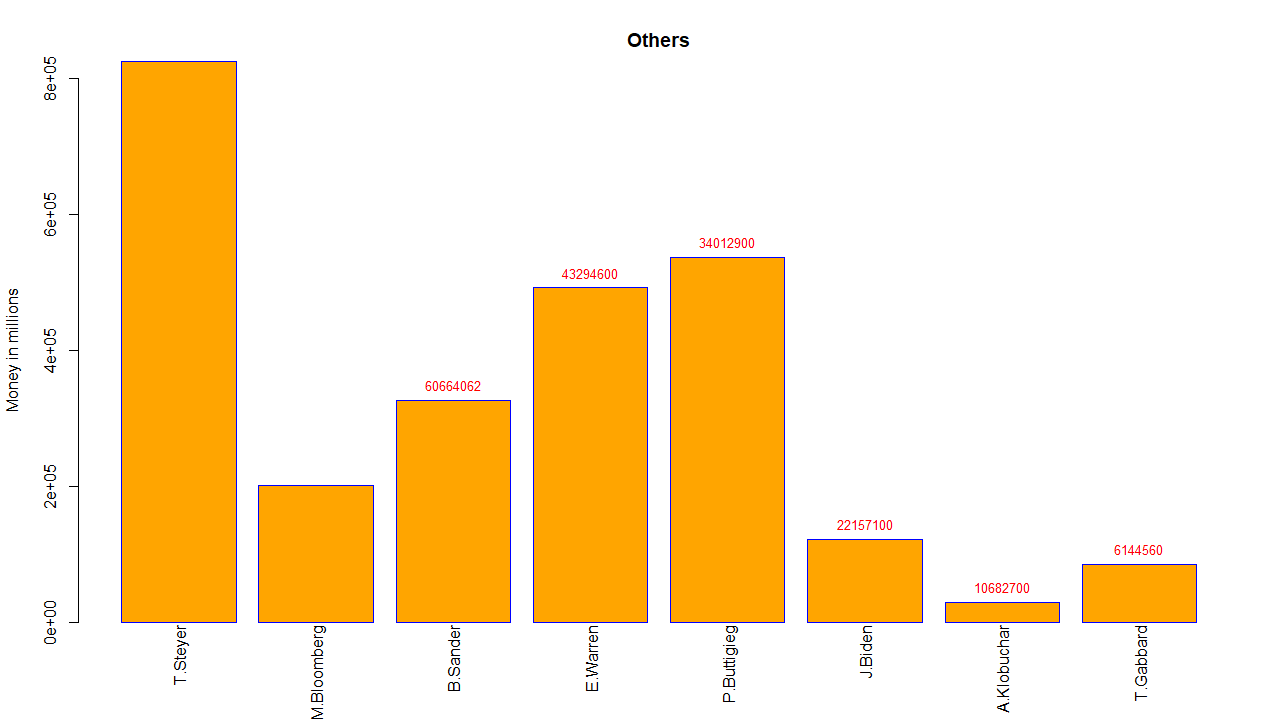
\includegraphics[width=0.9\textwidth]{figures/Others.png}
    \caption{Others Sources Funding}
    \label{Others}
\end{figure}
